%!Tex Root = ../Tutorat3.tex
% ./Packete.tex
% ./Design.tex
% ./Deklarationen.tex
% ./Aufgabe1.tex
% ./Aufgabe2.tex
% ./Aufgabe3.tex
% ./Aufgabe4.tex
% ./Bonus.tex

\section{Task 5}

\setcounter{task}{1}

\begin{frame}[allowframebreaks]{Task 5}{Earliest Deadline First – Star\vspace{0.5cm}}
  \begin{tasknoinc}
    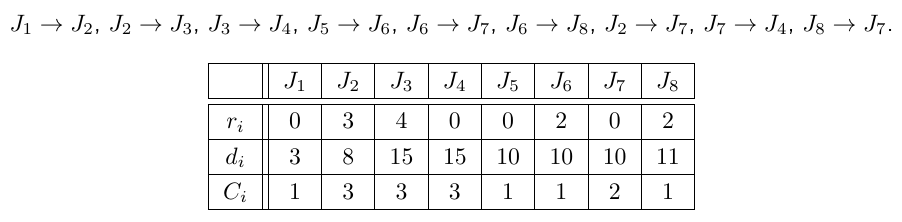
\includegraphics[width=\textwidth]{./figures/5_task.png}
    \begin{itemize}
      \item construct \alert{precedence graph}
    \end{itemize}
  \end{tasknoinc}
  \begin{solution}
    \centering
    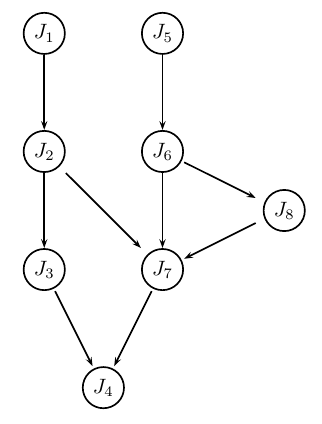
\includegraphics[width=0.3\textwidth]{./figures/5_graph.png}
  \end{solution}
\end{frame}

\begin{frame}[allowframebreaks]{Task 5}{Earliest Deadline First - Star\vspace{0.5cm}}
  \begin{tasknoinc}
    \begin{itemize}
      \item apply \alert{EDF* algorithm} for \alert{modified arrival times} and \alert{deadlines}
    \end{itemize}
    \centering
    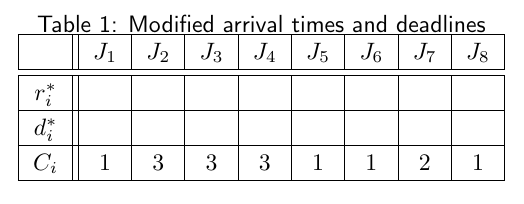
\includegraphics[width=0.5\textwidth]{./figures/5_table.png}
  \end{tasknoinc}
  \framebreak
    \begin{itemize}
        \item $r_1^* = r_1 = 0$, $r_5^* = r_5 = 0$
        \item $r_2^* = \max\{r_2,r_1^* + C_1\} = \max\{3, 0+1\} = 3$
        \item $r_6^* = \max\{r_6,r_5^* + C_5\} = \max\{2, 0+1\} = 2$
        \item $r_3^* = \max\{r_3, r_2^* + C_2\} = \max\{4, 3 + 3\} = 6$
        \item $r_8^* = \max\{r_8, r_6^* + C_6\} = \max\{2, 2 + 1\} = 3$
        \item $r_7^* = \max\{r_7,\max\{r_2^* + C_2, r_6^* + C_6, r_8^* + C_8\}\} = \max\{0, \max\{3 + 3, 2 + 1, 3 + 1\}\} = 6$
        \item $r_4^* = \max\{r_4,\max\{r_3^* + C_3, r_7^* + C_7\}\} = \max\{0, \max\{6 + 3, 6 + 2\}\} = 9$
    \end{itemize}
    \framebreak
    \begin{itemize}
        \item $d_4^* = d_4 = 15$
        \item $d_3^* = \min\{d_3, d_4^* - C_4\} = \min\{15, 15 - 3\} = 12$
        \item $d_7^* = \min\{d_7, d_4^* - C_4\} = \min\{10, 15 - 3\} = 10$
        \item $d_2^* = \min\{d_2, \min\{d_3^* - C_3, d_7^* - C_7\}\} = \min\{8, \min\{12-3, 10-2\}\} = 8$
        \item $d_1^* = \min\{d_1, d_2^* - C_2\} = \min\{3, 8 - 3\} = 3$
        \item $d_8^* = \min\{d_8, d_7^* - C_7\} = \min\{11, 10 - 2\} = 8$
        \item $d_6^* = \min\{d_6, \min\{d_7^* - C_7, d_8^* - C_8\}\} = \min\{10, \min\{10-2, 8-1\}\} = 7$
        \item $d_5^* = \min\{d_5, d_6^* - C_6\} = \min\{10, 7 - 1\} = 6$
    \end{itemize}
  \framebreak
  \begin{solution}
    \centering
    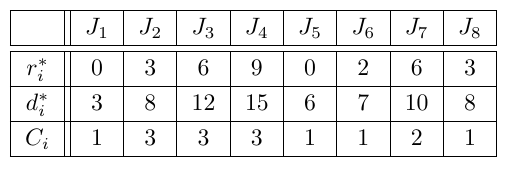
\includegraphics[width=0.5\textwidth]{./figures/5_table_sol.png}
  \end{solution}
\end{frame}

\begin{frame}[allowframebreaks]{Task 5}{Earliest Deadline First - Start\vspace{0.5cm}}
  \begin{tasknoinc}
    \begin{itemize}
      \item \alert{dual-core platform}
      \item at any time $t$, both cores execute the two ready tasks ($r_i* \le t$) with \alert{earliest deadlines}
      \item a single task \alert{cannot} be executed on two cores simultaneously
      \item construct schedule:
    \end{itemize}
  \end{tasknoinc}
  \begin{tasknoinc}
    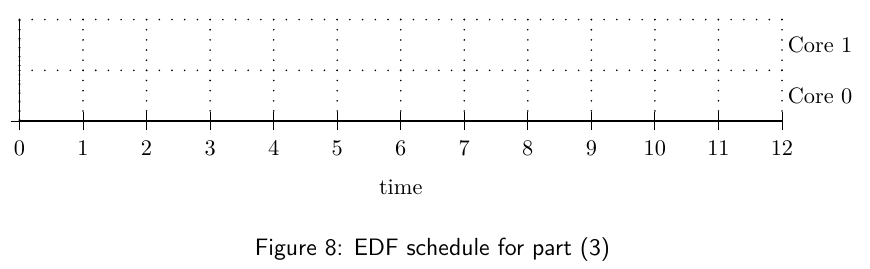
\includegraphics[width=\textwidth]{./figures/5_diag.png}
  \end{tasknoinc}
  \begin{solution}
    \begin{itemize}
      \item \alert{one of several solutions} since the tasks can run either on core 0 or core 1
    \end{itemize}
    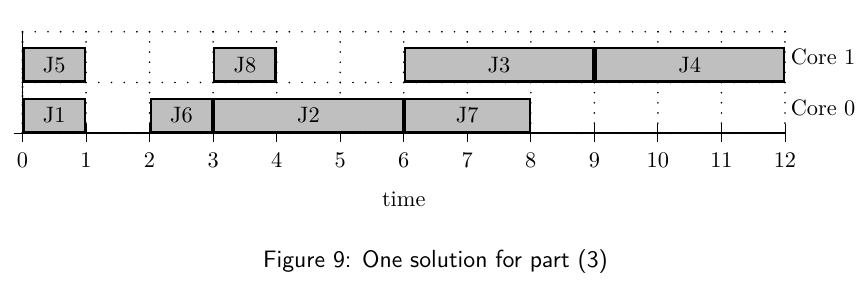
\includegraphics[width=\textwidth]{./figures/5_diag_sol.png}
  \end{solution}
\end{frame}

\begin{frame}[allowframebreaks]{Task 5}{Earliest Deadline First - Start\vspace{0.5cm}}
  \begin{tasknoinc}
    \begin{itemize}
      \item Will executing on the \alert{quad-core platform} with the same scheduling rule reduce the completion time of the application?
        \begin{itemize}
          \item $4$ cores execute the four ready tasks with earliest deadlines
        \end{itemize}
    \end{itemize}
  \end{tasknoinc}
  \begin{solution}
    \begin{itemize}
      \item No, $J_4$ \alert{cannot} be started earlier than time $9$. Therefore, the \alert{minimum finish time} of the application is $12$ (as the finish time for the dual core platform)
    \end{itemize}
  \end{solution}
\end{frame}
